\documentclass[11pt,conference]{IEEEtran}
\IEEEoverridecommandlockouts
% The preceding line is only needed to identify funding in the first footnote. If that is unneeded, please comment it out.
\usepackage{cite}
\usepackage{amsmath,amssymb,amsfonts}
\usepackage{algorithmic}
\usepackage{graphicx}
\usepackage{textcomp}
\usepackage{xcolor}
\usepackage{appendix}
%\usepackage{multirow}
\usepackage[lined,algonl,boxed]{algorithm2e}


\def\BibTeX{{\rm B\kern-.05em{\sc i\kern-.025em b}\kern-.08em
    T\kern-.1667em\lower.7ex\hbox{E}\kern-.125emX}}
\begin{document}




\title{ELEN4020: Data Intensive Computing\\ Matrix Transposition of Big-Data\\
{\footnotesize School of Electrical \& Information Engineering, University of the
Witwatersrand, Private Bag 3, 2050, Johannesburg, South Africa}
%\thanks{Identify applicable funding agency here. If none, delete this.}
}


\author{

\IEEEauthorblockN{Elias Sepuru 1427726}
\and
\IEEEauthorblockN{Boikanyo Radiokana 1386807}
\and
\IEEEauthorblockN{Lloyd Patsika 1041888}

}

\maketitle
\begin{abstract}
This report presents the implementation and analysis of matrix block transposition using straightforward MPI. The report divides the procedure into 4 main parts as follows: Input Data Generation of Matrices using Parallel I/O, Reading In of Data from Input Files using Parallel I/O and block transposition of matrices using MPI as well writing to files. The report anaylses the implementation through timing the various processes. It is noted that as the number of processors is increased, the time taken actually increases in most instances. Future recommendations include added code functionality which checks whether the transposition occurs properly, instead of human observation. Another improvement would be to provide another method of implementing parallelism in order to provide a more conclusive analysis.
\end{abstract}
\section{INTRODUCTION}
\noindent
Messaging-Passing Interface (MPI) is a versatile, standard interface for writing programs that run in parallel, using a distributed memory programming model. It is an interface which is generally used for composing parallel applications on systems such as laptops or clusters \cite{gropp2014using}.
\vspace{2mm}

\noindent
This report presents a block transposition implementation using Message-Passing-Interface in order to provide a comprehensive analysis of its performance. It involves the use of medium to large matrices being transposed through straight MPI with derived data types.

\section{BACKGROUND}
\noindent
 MPI was designed with large-scale systems in mind, and it is an architecture that supports highly parallel abstract machines through improving collective operations, scalable communicator and group operations. Reference \cite{10.1007/978-3-540-69389-5_29} states that MPI can be used in order to take advantage of massive parallel computation as MPI provides a framework for inter-process communication. This project used this functionality in order to achieve Parallel I/O as well as parallel implementation of block matrix transposition.
 
\subsection{Problem Description}
\noindent
The main problem that this report aims to solve is to develop and implement a parallel matrix transposition algorithm for very large data-sets that should be generated by a group of processors as sub-matrices but together form a large matrix file \cite{otto}. Furthermore, the matrix is required to be a large matrix A[N][N]. The input data, that is transposed after being read in, is initially in row major order after being generated by each submatrix using Parallel I/O. Another requirement is that the output data is also stored in row major order after transposition.

\subsection{Success Criteria}

\noindent
The success of the project depends on achieving the following:
\begin{itemize}
    \item Correct generation of the input data using Parallel I/O
    \item Correct storage of the input data in-out of core files
    \item Accurate Matrix Transposition using straight MPI
    \item Obtaining accurate time results for each important event, including input data generation, transposing of matrices and output data generation
\end{itemize}

\section{DESIGN \& IMPLEMENTATION}
\noindent
The Project is divided into 4 main parts: Generation of Matrices using random numbers, Reading of the generated input files, Transposition of the matrices and Writing of the transposed matrices to output files.


\subsection{Generation of Random Numbers and Writing to Files}
\noindent
The required matrices to be generated as input data include matrix dimensions of A[N][N], where N = \{8,16,32,64,128\}. The number of processors that should be used to perform this generation are P = \{16,32,64,128\}. 


\noindent
In general, the procedure for generation of data involved each sub-matrix being generated by a single process. Every process is responsible for the generation of its sub-matrix random numbers as well as writing these to the respective file. The sub matrices for each process are all equal and this means that they are assigned the same amount of memory as an offset. The process with rank 0 is also responsible for writing the matrix dimension. Algorithm 1 shows the general pseudo code for this procedure.

\linesnumbered
\begin{algorithm}[h!]

\centring

\SetKwData{in}{in}
\SetKwData{not}{not}
\SetKwData{st}{\texttt{StopWords}}
\SetKwInOut{Input}{input}
\SetKwInOut{Output}{output}
\SetKwFunction{wi}{WordIndex(mrs.MapReduce)}
\SetKwFunction{red}{reduce(word,line\_num)}
\SetKwFunction{mpiFileO}{MPI\_File filehandler}
\SetKwFunction{mpiStatus}{MPI\_Status status}
\SetKwFunction{mpiComm}{MPI\_Comm comm}
\SetKwFunction{mpiI}{MPI\_Init}
\SetKwFunction{mpiFileOpen}{MPI\_File\_open}
\SetKwFunction{c}{MPI\_COMM\_WORLD}
\SetKwFunction{n}{file\_name}
\SetKwFunction{mpiOff}{MPI\_Offset}
\SetKwFunction{abort}{MPI\_Abort}
\SetKwFunction{cs}{MPI\_Comm\_size}
\SetKwFunction{crr}{MPI\_Comm\_rank}
\SetKwFunction{setV}{MPI\_File\_set\_view}
\SetKwFunction{finalize}{MPI\_Finalize\(\)}




\caption{\texttt{Matrix Generation using MPI}}
\Input{The dimension of the matrix to be generated}
\Output{Text file with Output Matrix}
\vspace{0.5cm}

\mpiFileO\\
\mpiStatus\\
\mpiComm\\
\mpiI\\


 \For{i \in MatrixDimension}
     {
     \emph{Creating the filename}
     file\_name$\leftarrow$ "file\_"+"MatrixDimension"
     \ error$\leftarrow$MPI\_File\_open(comm, n, MPI\_MODE\_RDONLY, MPI\_INFO\_NULL,\&filehandler)
     \mpiOff offset \leftarrow 0 \\
     \If{error}{\abort (\c,911)}
     \cs(comm,\&size)\\
     \crr (comm, \&process\_rank)\\
     \emph{Writing MatrixDimension at Position 0} \\
     \If{process\_rank EQUALS 0}{ \mpiOff temp \leftarrow 1 \\
        error$\leftarrow$MPI\_File\_write(comm, n, MPI\_MODE\_RDONLY, MPI\_INFO\_NULL,\&filehandler)}
         \emph{Dividing Matrix into Chunks}
    \mpiOff chunk\_memory \leftarrow (MatrixDimension\times MatrixDimension/size)\\
    randomNumbersBuffer \leftarrow chunk\_memory \times sizeof(int)\\
    randomNumberGenerator(randomNumbersBuffer\\,chunk\_memory)\\
    \emph{Calculating Offset based on memory}\\
    offset \leftarrow ((process\_rank\times chunk\_memory)+1)\times sizeof(int)\\
    \setV (filehandler,offset,MPI_INT,MPI_INT,"native",\\ MPI\_INFO\_NULL)
    error \leftarrow MPI\_File\_write\_all(filehandler,\\randomNumbersBuffer,chunk\_memory,MPI\_INT, \&status_)
    error \leftarrow MPI\_File\_close (\&filehandler)\\
     }
\finalize
\label{ii}
\end{algorithm}



\subsection{Reading of the Input Data}
\noindent
An input text file is read in, in order to access the data, for transposition. The process is quite similar to the one for writing as each process is given a position in the input text file to read from. The processes then read their sub matrices and put them at specific positions in a 1D array. In order to have the data ready for transposition, the 1D array components are then transferred into a 2D array.

\subsection{Matrix Transposition}
\noindent
Matrix transposition is performed using the \texttt{MPI\_Alltoall} function together with the  \texttt{localTrans()} function. \texttt{MPI\_Alltoall} sends data from all processors to all processors. In other words, it sends distinct data to all the processes that are receivers \cite{1}. This exchange of data from one process to another yields an outer matrix block transposition of elements. \texttt{MPI\_Alltoall} achieves this process by sending a block of data (block \textit{j}) from process \textit{i} to the recieve buffer of process \textit{j}. In the receive buffer of process \textit{j}, the received block is placed in the i$^{th}$ block. The \texttt{MPI\_Alltoall} function takes the data types of the sender and receiver, \texttt{MPI\_COMM\_WORLD} function, the number of elements sent and the elements that the receiver is accepting. For matrix transposition to be successful, the amount of data sent by process \textit{i} must be the same as the amount of data received by process \textit{j}, however the type of maps can be different. The \texttt{MPI\_COMM\_WORLD} argument is a communicator that groups together all processes at the beginning of the program to ensure that processes can communicate with each other \cite{2}. Communication can be achieved in two ways, namely \cite{2}:
\begin{itemize}
    \item Point-to-point Communication
    \item Collective Communication
\end{itemize}
Collective communication was used because it allows all processes to communicate collectively. Figure 1 shows how the processes can communicate.

\begin{figure}[h!]
    \centering
    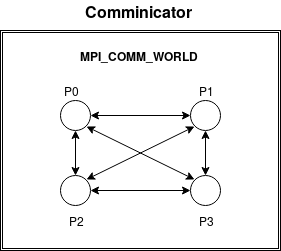
\includegraphics[scale=0.4]{world.png}
    \caption{Collective communication in MPI\_COMM\_WORLD}
    \label{7}
\end{figure}

\noindent
Following the transposition of the outer blocks with \texttt{MPI\_Alltoall}, the \texttt{localTrans()} function transposes the local elements of the blocks within each process. This is done in parallel for all processes. Algorithm 2 shows the pseudo code used to transpose the elements within each process.

\begin{algorithm}[h!]


\SetKwData{temp}{temp}
\SetKwData{otherCol}{otherCol}
\SetKwData{otherRow}{otherRow}
\SetKwData{A}{A}
\SetKwFunction{swap}{swap}
%\SetKwFunction{FindCompress}{FindCompress}
\SetKwInOut{Input}{input}
%\SetKwInOut{Output}{output}
\caption{\texttt{blockElementTranspose(A)}}\Input{A 2D matrix "A" of size $n\times n$}

\otherCol$\leftarrow$0
\\
\otherRow$\leftarrow$0

%\Output{A resultant C 2D matrix}
%%\BlankLine\emph{special treatment of the first line}\;
\For{$i\gets0$ \KwTo $n-1$}{
\For{$j\gets0$ \KwTo $n-1$}{
%\emph{special treatment of the first element of line $i$}\;
     \For{$k\gets{0}$ \KwTo $BLOCK\_SIZE$}{
%\nllabel{forins}
          \For{$l\gets{0}$ \KwTo $l < k$}{
         
            \If{$i != j$}{
                   \otherRow$\leftarrow(i + l)$
                   \otherCol$\leftarrow(j + k)$   
               }
              \Else{
                    \otherRow$\leftarrow(l+j)$
                    \otherCol$\leftarrow(k+i)$   
                  }
          
            
           \swap($A[k+i][l+j]$, $A[\otherRow][\otherCol]$)
            }
}

}
}

\label{block}
\end{algorithm}


\subsection{Output Data Generation}
\noindent
Each process is responsible for writing its sub matrix to a file. The process is quite similar to the one for writing of random numbers to a file as each process is given a position in the output text file to write to. The processes then write their sub matrices at specific positions in the output text file. The output file then contains all matrix values which were contained in all the sub matrices of the process once the process is complete. These values are stored in row-major order, as required.
\section{CRITICAL ANALYSIS}

\subsection{Environment Used}
\noindent
The programs are coded in C. In order to allow for proper testing of the code, {\sl hornet01.eie.wits.ac.za} is the cluster that is used. The cluster has a memory size of 16GB and a 3.4GHz. Although the cluster has 373 processors, a maximum number of 128 is used for this project. The environment has an MPI version called MPICH3.3.


\subsection{Results}
\noindent
Figures 2-3 show graphs of program performances. A general trend shown is that the number of processors used does not correlate to a shorter time for execution. The results follow Amdahl's Law. It re-affirms the idea that an increase in the processor number does not necessarily mean a faster execution time.

% Please add the following required packages to your document preamble:
\begin{figure}[h!]
    \centering
    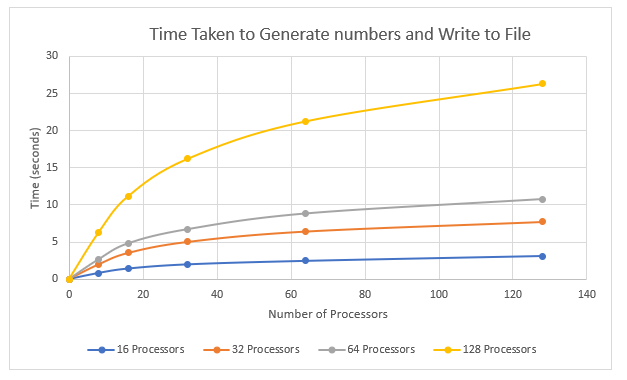
\includegraphics[scale=0.52]{input.PNG}
    \caption{Time Taken to Generate Input Data}
    \label{7}
\end{figure}

\begin{figure}[h!]
    \centering
    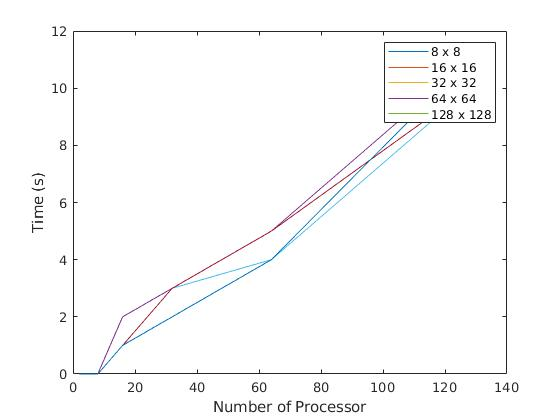
\includegraphics[scale=0.5]{out.jpg}
    \caption{Time Taken to Transpose Matrices and Write to File}
    \label{7}
\end{figure}




\subsection{Future Recommendations}
\noindent
As an improvement to the project, it is recommended that another method such as UPC or UPC++ be used in order to compare to the method used in this project. This is because, although this project makes use of timing in order to compare one algorithm at different processes and matrix sizes, it would be much better research if there was another method that is able to also transpose matrices for purposes of comparison. Another recommendation which would improve the functioning of the program would be the addition of functionality to check the validity of the transpose.
\section{Work Division}
\noindent
The project was divided into manageable tasks and delegated amongst the members of the team. The team members,Elias Sepuru, Boikanyo Radiokana and Lloyd Patsika are final year  Electrical and Information Engineering students. The following table shows the work division between the members mentioned:
\begin{table}[h!]
\caption{Work division among team members}
\label{divison}
\begin{tabular}{|l|l|l|l|}
\hline
\multicolumn{4}{|c|}{\textbf{Work Division}} \\ \hline
\textbf{Elias Sepuru} & \multicolumn{3}{l|}{\begin{tabular}[c]{@{}l@{}}Code: Matrix transposition, Integration \\ of all codes and Timing \\ Report: Section 3B, Section 4A,\\  Section 4B\end{tabular}} \\ \hline
\textbf{Boikanyo Radiokana} & \multicolumn{3}{l|}{\begin{tabular}[c]{@{}l@{}}Code: Writing from a file, Integration  of all\\ codes and TimingReport: Section 3A, Section 5,\\  Conclusion\end{tabular}} \\ \hline
\textbf{Lloyd Patsika} & \multicolumn{3}{l|}{\begin{tabular}[c]{@{}l@{}}Code: Random number generation and \\ Reading to the file, Integration \\ of all codes and Timing\\ Report: Introduction, Background, \\ Section 3C\end{tabular}} \\ \hline
\end{tabular}
\end{table}

\section{CONCLUSION}
\noindent
A straightforward MPI implementation is presented, where matrix block transposition is implemented in order to critically analyse its performance. The different size matrices are generated using Parallel I/O. This parallel implementation also extends to the reading of input files as well as the writing of the results generated by the transposition. Timing was used in order to analyse the performance of the program and it was noted that an increase in the number of processors does not necessarily correlate to an decrease in the time for execution of the program. Recommendations to improve the code include implementing another form of parallelism using UPC/UPC++ while necessary changes to the code include code tests to confirm accurate transposition.


\onecolumn
\newpage

\bibliography{sample.bib}
\bibliographystyle{ieeetr}

\onecolumn
\appendix
\setcounter{page}{1}
\setcounter{equation}{0}
\setcounter{figure}{0}
\setcounter{table}{0}
\setcounter{section}{0}
\setcounter{algorithm}{0}

\subsection{Graphs showing various times of execution of code}

\begin{table}[h!]
\centering
\caption{Time taken for Input Generation and Writing to Files}
\label{tab:my-table}
\begin{tabular}{|l|l|l|l|l|}
\hline
\textbf{Matrix Sizes} & \textbf{16 Pro.} & \textbf{32 Proc.} & \textbf{64 Proc.} & \textbf{128 Proc.} \\ \hline
8 & 0,829196s & 1,997403s & 2,675249s & 6,30365s \\ \hline
16 & 1,425108s & 3,55822s & 4,831607s & 11,183438s \\ \hline
32 & 1,989904s & 5,049717s & 6,731276s & 16,201182s \\ \hline
64 & 2,465029s & 6,466829s & 8,855374s & 21,271032s \\ \hline
128 & 3,126022s & 7,772867s & 10,802833s & 26,308761s \\ \hline
\end{tabular}
\end{table}

% Please add the following required packages to your document preamble:
% \usepackage{graphicx}
\begin{table}[h!]
\centering
\caption{Time taken for Transposition and Writing to Files}
\label{tab:my-table}
\resizebox{\textwidth}{!}{%
\begin{tabular}{|l|l|l|l|l|l|l|l|}
\hline
\textbf{Matrix Sizes} & \textbf{2 Pro.} & \textbf{4 Proc.} & \textbf{8 Proc.} & \textbf{16 Proc.} & \textbf{32 Proc.} & \textbf{64 Proc.} & \textbf{128 Proc.} \\ \hline
8 & 0s & 0s & 0s & 2s & 3s & 5s & 11s \\ \hline
16 & 0s & 0s & 0s & 1s & 2s & 4s & 10s \\ \hline
32 & 0s & 0s & 0s & 1s & 3s & 4s & 10s \\ \hline
64 & 0s & 0s & 0s & 1s & 3s & 5s & 10s \\ \hline
128 & 0s & 0s & 0s & 1s & 2s & 4s & 11s \\ \hline
\end{tabular}%
}
\end{table}


\newpage
%%%%%%%%%%%%%%%%%%%%%%%%%%%%%%%%%%%%%%%%%%%%%%%%%%%%%%%%%%%%%%%%%%%%%%%%%%%%%%%%%%%%%%%%%%%%%%%%%5
\begin{algorithm}[h]
\SetKwData{in}{in}
\SetKwData{out}{out}
\SetKwData{rank}{rank}
\SetKwData{numProcs}{numProcs}
\SetKwData{inputError}{inputError}
\SetKwData{SIZE}{SIZE}
\SetKwData{sizeChecker}{sizeChecker}
\SetKwData{tempBuffer}{tempBuffer}
\SetKwData{n}{n}
\SetKwFunction{file}{MPI\_File }
\SetKwFunction{win}{MPI\_Win }
\SetKwFunction{status}{MPI\_Status }
\SetKwFunction{disp}{MPI\_Offset}
\SetKwFunction{a}{blocksize}
\SetKwFunction{c}{MPI\_Init}
\SetKwFunction{d}{MPI\_Comm}
\SetKwFunction{e}{MPI\_Comm\_size}
\SetKwFunction{f}{MPI\_File\_set\_view}
\SetKwFunction{g}{MPI\_File\_read}
\SetKwFunction{h}{MPI\_File\_Close}


%%%%

%\SetKwFunction{FindCompress}{FindCompress}
\SetKwInOut{Input}{input}
%\SetKwInOut{Output}{output}
\caption{\texttt{blockElementTranspose(A)}}

\emph{\textbf{Initialize MPI}}\\
\c(\&argc, \&argv)\\
\d(MPI\_COMM\_WORLD, \&rank) \\
\e (MPI\_COMM\_WORLD, \&numProcs) \\

\emph{\textbf{MPI Setup}}\\
\file fh \\
\win win \\
\status status \\
\disp disp\\
\disp blocksize \\
\vspace{0.5cm}
\emph{\textbf{Open file}}\\
\ inputError$\leftarrow$MPI\_File\_open(MPI\_COMM\_WORLD, in, MPI\_MODE\_RDONLY, MPI\_INFO\_NULL,\&fh)
\vspace{0.5cm} \\ 
\emph{\textbf{Validate file open successfully}} \\
\If{inputError}{
    \If{\rank$\leftarrow$0}{
    \ Display Error \\
    \ MPI\_Finalize() \\
    \ exit()
    }
}
\vspace{0.5cm} \\
\emph{\textbf{Get size of matrix}}\\

\ sizeChecker$\leftarrow$ 1 byte \\
\ \file(fh, sizeChecker, 1, MPI\_INT, \&status) \\
\ SIZE$\leftarrow$\sizeChecker[0] \\
\ Display the SIZE \\
\ Free memory of \sizeChecker \\
\ n$\leftarrow$ SIZE divide by numProcs
\vspace{0.5cm} \\
\emph{\textbf{Condition buffer for each rank}}\\
\ blockSize$\leftarrow$ SIZE \times n \\
\ disp$\leftarrow$(rank\times blockSize)+1 \times sizeof(int) \\
\ tempBuffer$\leftarrow$ (int*)malloc(sizeof(int)) \\
\vspace{0.5cm} \\
\emph{\textbf{Read file into Buffer}}\\
\f (fh, disp, MPI\_INT, MPI\_INT, "native", MPI\_INFO\_NULL)\\
\g (fh, tempBuffer, blocksize, MPI\_INT, \&status)\\
\h (\&fh)\\
\vspace{0.5cm} \\
\emph{\textbf{Confirm}}\\
\For{i$\leftarrow$ blocksize}{
    \If{\rank$\leftarrow$1}{
    Display rank and tempBuffer[i] }

}

\label{block}
\end{algorithm}

%%%%%%%%%%%%%%%%%%%%%%%%%%%%%%%%%%%%%%%%%%%%%%%%%%%%%%%%%%%%%%%%%%%%%%%%555



\end{document}
